The firmware to control the OCCs has been updated over the last year as data requirements have changed and the ability to use more precise timing increments have became available. Testing the updated firmware versions has been essential to confirm uniformity in the data collected between versions. In this section the testing procedure, firmware changes and results will be discussed.

\section{Full system test}
During each full system test (FST) the optical calibration cards are inserted into a VME crate and is connected to a computer via USB for control, as seen in figure \ref{fig:TestStand}. On the computer a python script is used to control the testing procedure. The process of testing is fully automated and initiated with the user inputting scan settings. The python scripts start the test with a given set pulse widths, pulse frequency and constants. The control commands and test settings are sent from the computer using a set of predefined registers to the OCC and interpreted by the FPGA motherboard. The FPGA chip controls the pulser board to pulse the light with pre-defined settings. The FPGA motherboard also sends the pulse width and pulse frequency to the oscilloscope for visual interpretation. Light from the pulser board is split down three optical fibres using an optical coupler. The first optical fibre is connected to a photo-diode board and the output is read back to the computer via the FPGA motherboard. The second optical fibre is connected to a power meter and this output is read back directly to the computer by USB. The third optical fibre is connected to a Hamamatsu H10721 PMT. The PMT is connected to the oscilloscope for visual interpretation. A DRS4 Evaluation Board is used to digitise the PMT pulses and FPGA board triggers at 5 Giga samples per second. Data from the DRS4 is read back directly to the computer by USB \cite{DRS4}. An Arudino board is used to control the gain of the PMT controlled from the python script. The test stand is setup such that only one channel can be tested at any one time. A schematic of the test stand can be seen in figure \ref{fig:FST_Flow}. The following list illustrates the data taken on each test:

\begin{itemize}\label{list:FSTdata}
    \item Number of photons per pulse with error
    \item Time on system clock
    \item Trigger width
    \item Trigger amplitude
    \item Position of the trigger peak
    \item Pulse width
    \item Pulse amplitude
    \item Position of pulse peak
    \item Width set
\end{itemize}

\begin{figure}[h]
    \centering
    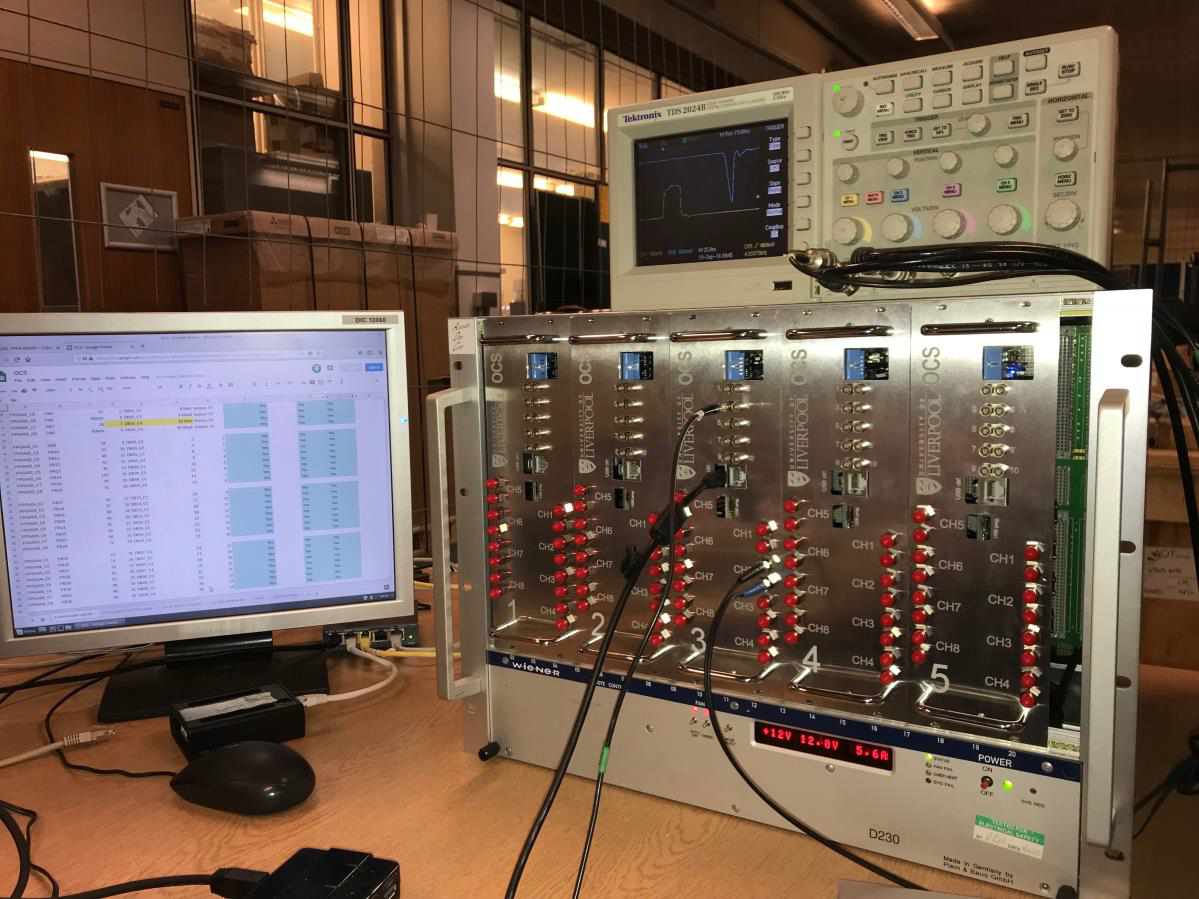
\includegraphics[width=0.7\textwidth]{Figures/TestStand.png}
    \caption{Test stand with the OCCs placed in the VME crate and oscilloscope connected for testing.}
    \label{fig:TestStand}
\end{figure}

\begin{figure}[h!]
    \centering
    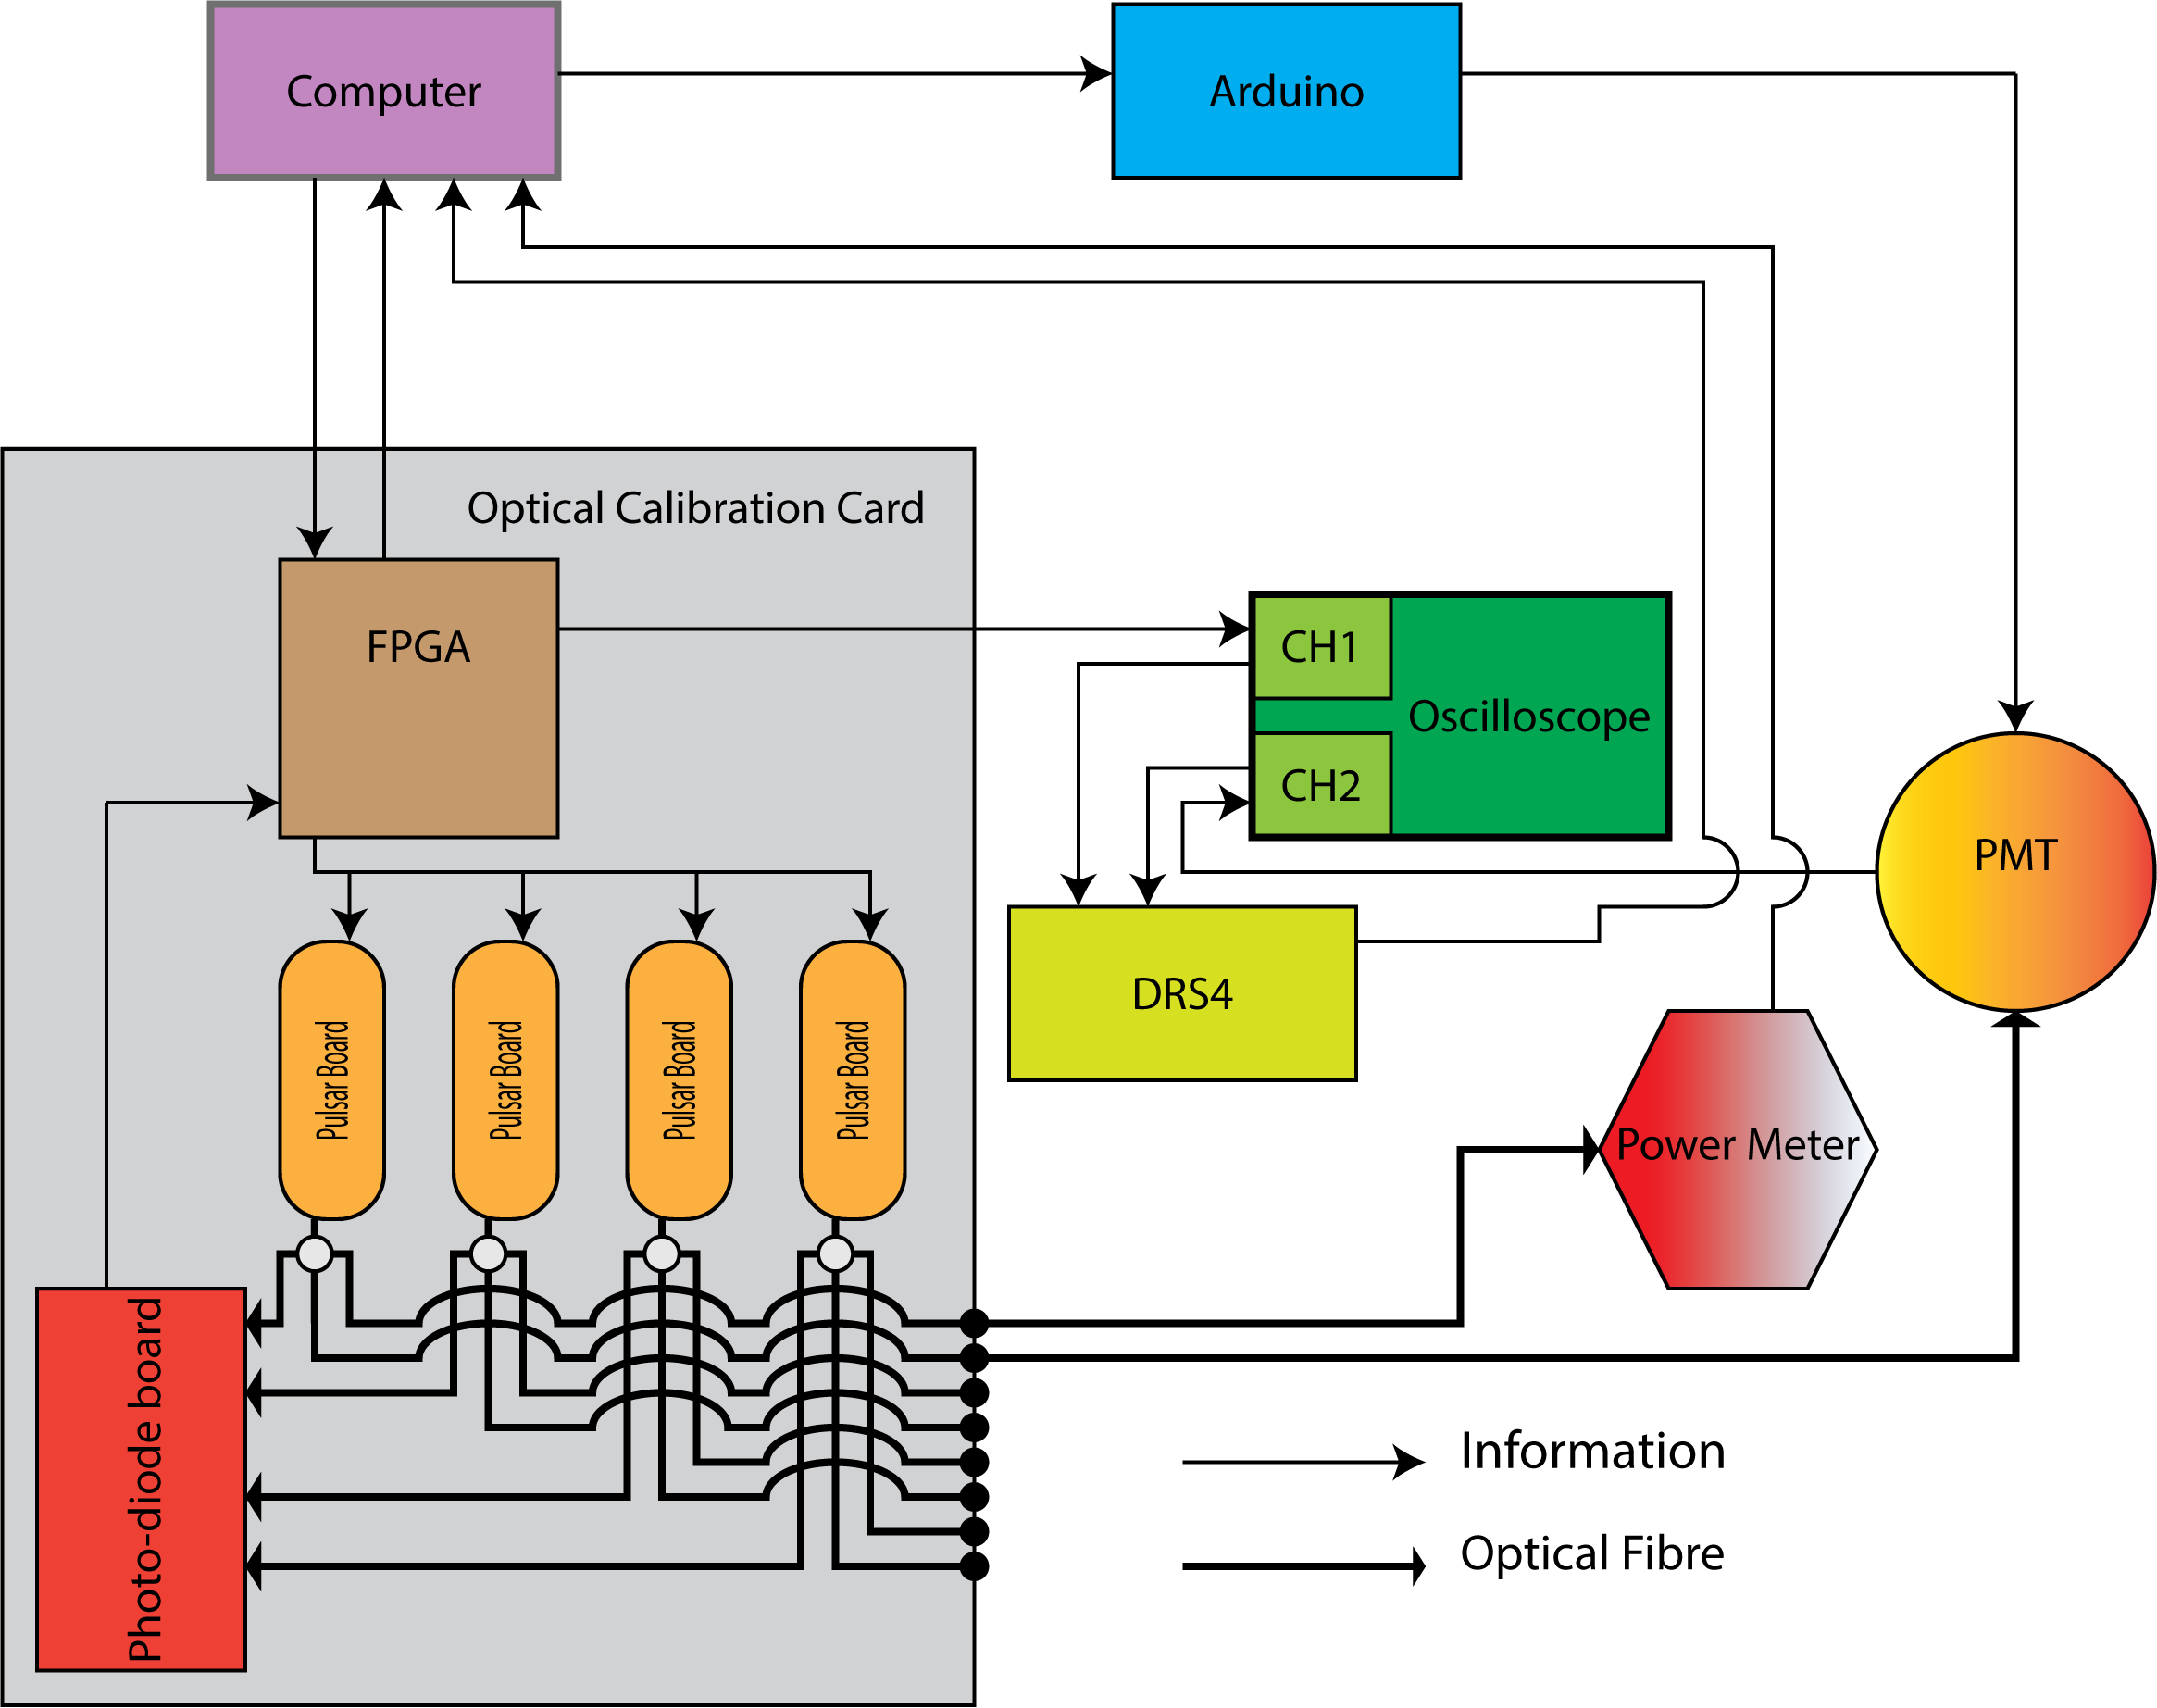
\includegraphics[width=0.7\textwidth]{Figures/FST.png}
    \caption{Schematic of the FST on a channel by channel test schedule. One board has been shown to demonstrate the process, showing the front side on an OCC. The remaining pulser boards and photo-diode board are located on the rear of the OCC.}
    \label{fig:FST_Flow}
\end{figure}

\section{Results}
After each OCC firmware update a full system test was conducted to confirm that the changes made to the firmware work correctly and to check the uniformity between firmware versions. Only one OCC was used throughout the testing as the firmware was updated, this decision was made due to time constraints. The data sets which were checked between firmware updates are: trigger width; pulse width; and width set. These data sets were monitored due to the changes which were made in the firmware. The data presented in the following subsections is from tests conducted on OCC-2 Channel 2 corresponding to pulser board 10.
\subsection{Trigger width}\label{subsec:trigw}
The Trigger Width (TW) is the measured width of the electronic pulse which is sent to the pulser board in order to produce light from the LED. TW is plotted against the natural logarithm of the number of photons per pulse (lnNph) in figure \ref{fig:trigw}. Figures \ref{fig:trig1},\ref{fig:trig2} and \ref{fig:trig3} have been fitted with the equation \ref{eqn:trigfit} where A, B and C correspond to calibration coefficients.  
\begin{equation}
    TW = A + e^{Bln(Nph)^2 + Cln(Nph))}
\label{eqn:trigfit}
\end{equation}
The optical calibration program will utilise equation \ref{eqn:trigfit} to determine the trigger width needed when a user defines the number of photons to inject into the OD. Equation \ref{eqn:trigfit} is currently being adapted to fit to the more complex curve produced by the data seen in figure \ref{fig:trig4}. In firmware version 1 and version 2, a $\sim5ns$ step in trigger width was used for faster testing capabilities in early tests. In firmware version 3 and version 4, a $\sim75ps$ step in the trigger width was implemented, utilising the full capability of the FPGA motherboard. Decreasing the step in trigger width measurements allows for more data points within the given trigger width range, this results in a fit function which represents the data more precisely. 
\newline
The equation fitted to the data has not been developed throughout the firmware updates. As the number of data points has increased the equation will be developed to reduce the $\chi^2$ value associated with the fit. 
\newline
As discussed early, the fit function will be used in the OCS to determine the trigger width corresponding to a specific number of photons, so the accuracy of the function is paramount. 

\begin{figure}[ht!]
\centering
    \begin{subfigure}[b]{.475\textwidth}
        \centering
        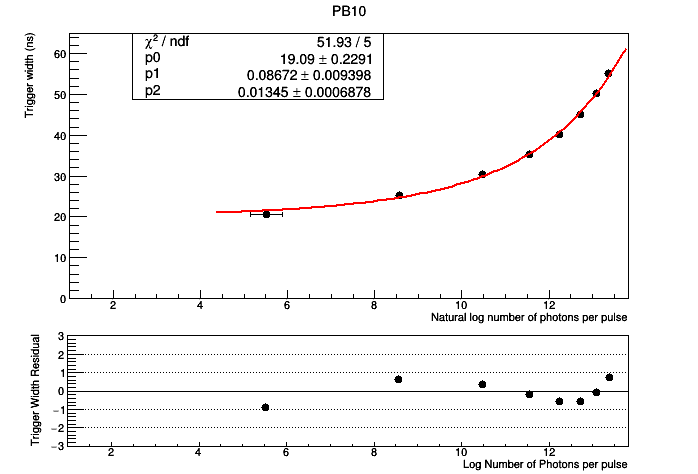
\includegraphics[width=\textwidth]{Figures/Plots/V1_ln(Nph)vsTriggerWidthResidual.png}
        \caption{Firmware version 1.}
        \label{fig:trig1}
    \end{subfigure}
    \hfill
    \begin{subfigure}[b]{.475\textwidth}
        \centering
        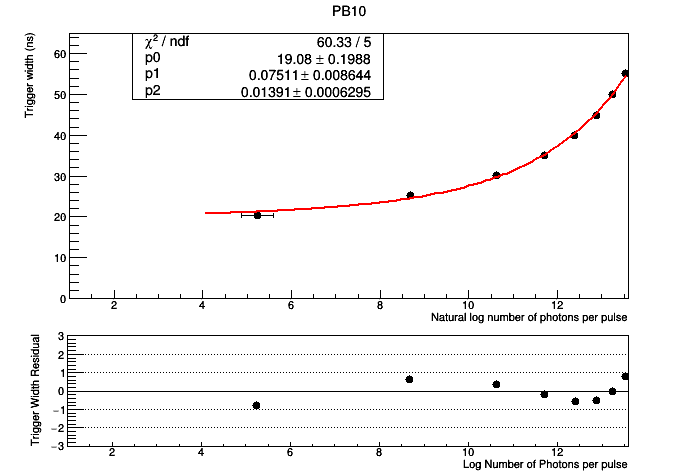
\includegraphics[width=\textwidth]{Figures/Plots/V2_ln(Nph)vsTriggerWidthResidual.png}
        \caption{Firmware version 2.}
        \label{fig:trig2}
    \end{subfigure}
    \vskip\baselineskip
    \begin{subfigure}[b]{.475\textwidth}
        \centering
        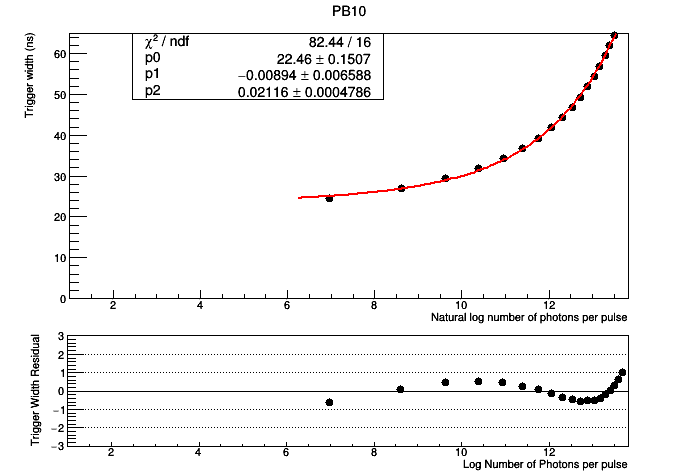
\includegraphics[width=\textwidth]{Figures/Plots/V3_ln(Nph)vsTriggerWidthResidual.png}
        \caption{Firmware version 3.}
        \label{fig:trig3}
    \end{subfigure}
    \hfill
    \begin{subfigure}[b]{.475\textwidth}
        \centering
        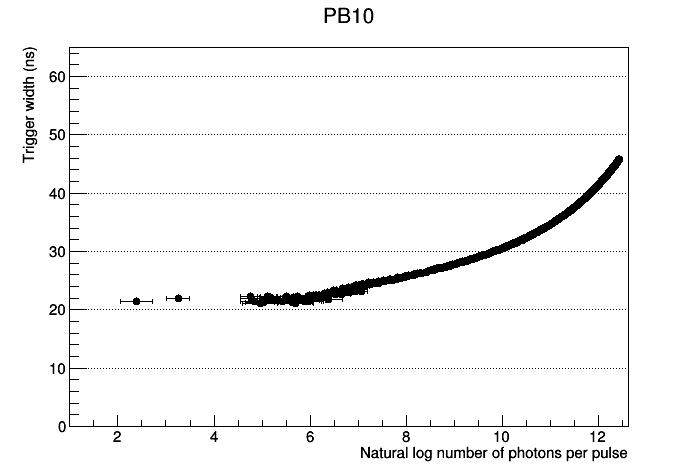
\includegraphics[width=\textwidth]{Figures/Plots/V4_ln(Nph)VSTriggerWidthPB10.png}
        \caption{Firmware version 4.}
        \label{fig:trig4}
    \end{subfigure}
    \caption{The evolution of the trigger widths measured as the OCC firmware was updated. The natural logarithm of the number of photons per pulse was used to aid the fitting the calibration curve to the plot. The fit residual is plotted below each plot where the data has been fitted with the equation \ref{eqn:trigfit}.}
    \label{fig:trigw}
\end{figure}



\subsection{Pulse width}\label{subsec:pulsew}
The Pulse Width is the measured taking the full width at half peak maximum of the light pulse which is detected by the PMT. Pulse width is monitored between firmware versions to ensure the system meets the requirements set by LZ (\ref{list:SystemReq}). Pulse Width is plotted against the logarithm of the number of photons per pulse in figure \ref{fig:trigw}.  
\begin{figure}[ht!]
\centering
    \begin{subfigure}[b]{.475\textwidth}
        \centering
        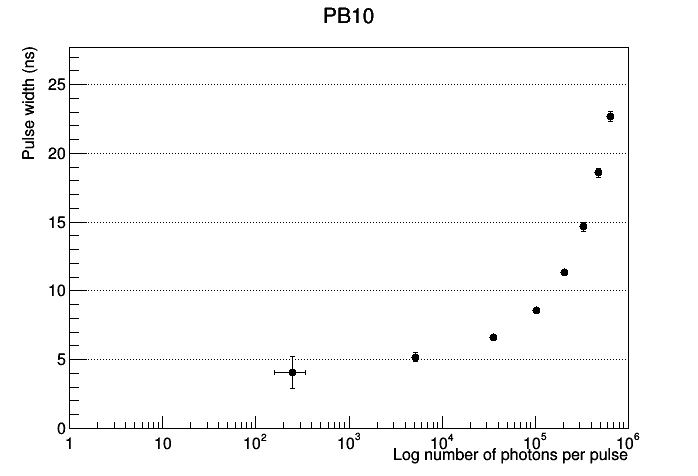
\includegraphics[width=\textwidth]{Figures/Plots/V1_log(Nph)vsPulseWidthPB10.png}
        \caption{Firmware version 1.}
        \label{fig:pulse1}
    \end{subfigure}
    \hfill
    \begin{subfigure}[b]{.475\textwidth}
        \centering
        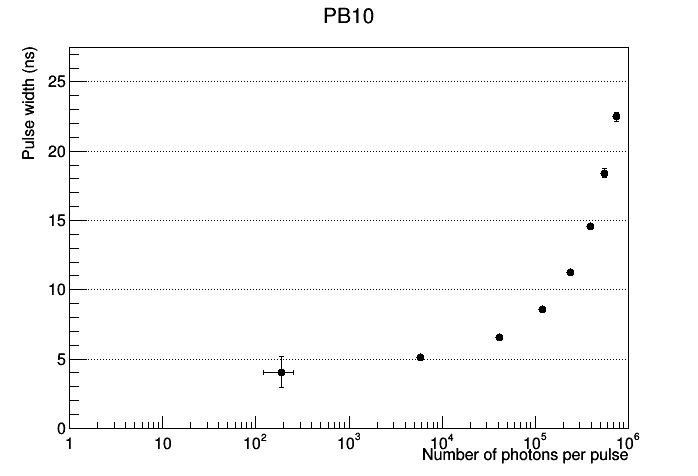
\includegraphics[width=\textwidth]{Figures/Plots/V2_log(Nph)vsPulseWidthPB10.png}
        \caption{Firmware version 2.}
        \label{fig:pulse2}
    \end{subfigure}
    \vskip\baselineskip
    \begin{subfigure}[b]{.475\textwidth}
        \centering
        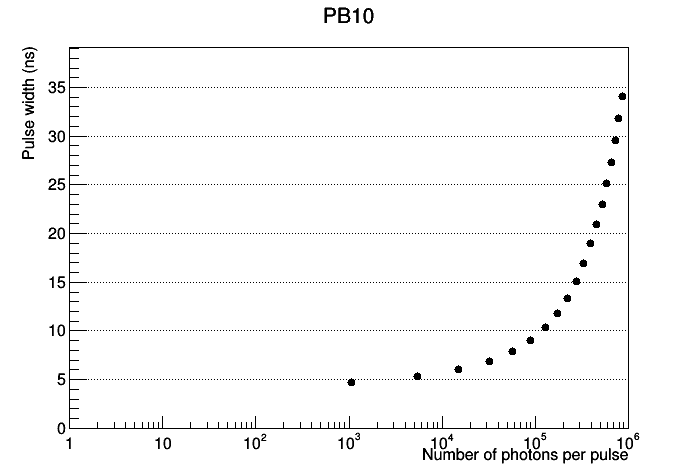
\includegraphics[width=\textwidth]{Figures/Plots/V3_log(Nph)vsPulseWidthPB10.png}
        \caption{Firmware version 3.}
        \label{fig:pulse3}
    \end{subfigure}
    \hfill
    \begin{subfigure}[b]{.475\textwidth}
        \centering
        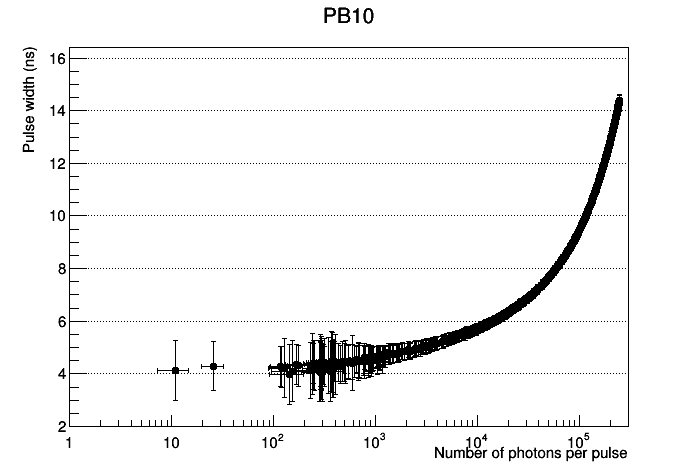
\includegraphics[width=\textwidth]{Figures/Plots/V4_log(Nph)VSPulseWidthPB10.png}
        \caption{Firmware version 4.}
        \label{fig:pulse4}
    \end{subfigure}
    \caption{Evolution of the pulse widths measured as the OCC firmware was updated. The logarithm of the number of photons per pulse is plotted against the pulse width.}
    \label{fig:pulsew}
\end{figure}
\subsection{Width set}\label{subsec:widthset}
The width set values correspond to scan points throughout the testing. As discussed in subsection \ref{subsec:trigw}, in firmware versions 1 and 2 a trigger width step of $\sim5ns$ was implemented resulting in the testing of 8 scan points. In testing firmware version 3, 19 points were scanned. In firmware version 4, 640 points were scanned. The increase in scan points between versions was due to the change in trigger width step. In firmware version 4, 10 large width set points were used with each large width set step containing 64 small width set points. Width set was monitored between firmware versions as the values used for iteration within scripts to produced the plots in figures \ref{fig:trigw},\ref{fig:pulsew} and \ref{fig:widthset}.
\begin{figure}[ht!]
\centering
    \begin{subfigure}[b]{.475\linewidth}
        \centering
        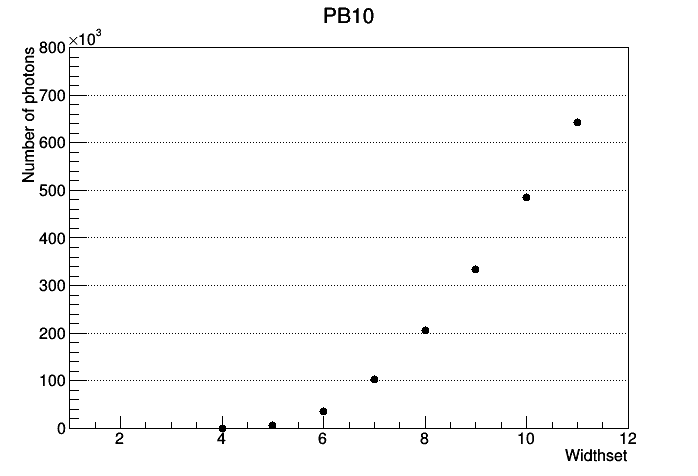
\includegraphics[width=\textwidth]{Figures/Plots/V1_widthsetVSNphPB10.png}
        \caption{Firmware version 1.}
        \label{fig:width1}
    \end{subfigure}
    \hfill
    \begin{subfigure}[b]{.475\linewidth}
        \centering
        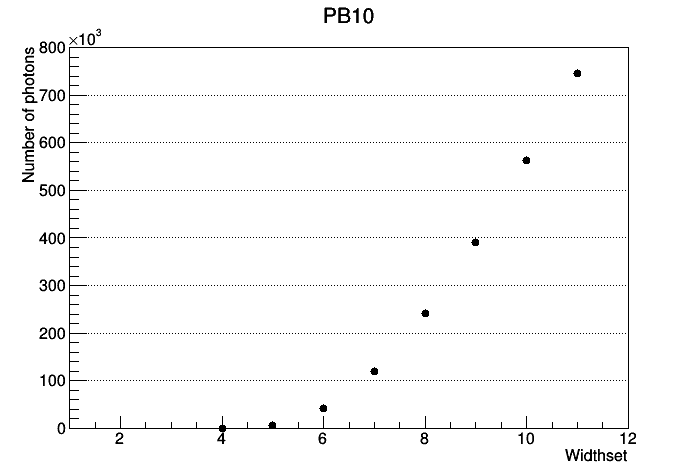
\includegraphics[width=\textwidth]{Figures/Plots/V2_widthsetVSNphPB10.png}
        \caption{Firmware version 2.}
        \label{fig:width2}
    \end{subfigure}
    \vskip\baselineskip
    \begin{subfigure}[b]{.475\linewidth}
        \centering
        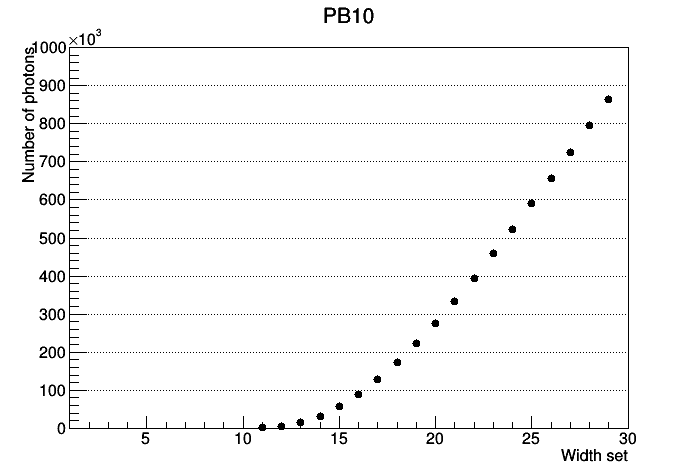
\includegraphics[width=\textwidth]{Figures/Plots/V3_widthsetVSNphPB10.png}
        \caption{Firmware version 3.}
        \label{fig:width3}
    \end{subfigure}
    \hfill
    \begin{subfigure}[b]{.475\linewidth}
        \centering
        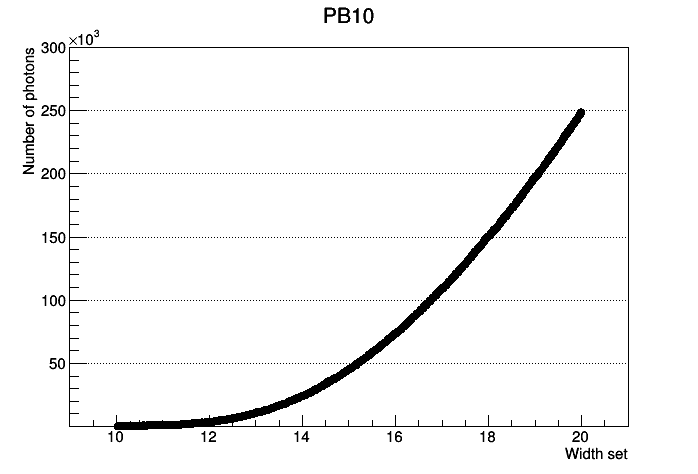
\includegraphics[width=\textwidth]{Figures/Plots/V4_widthsetVSNphPB10.png}
        \caption{Firmware version 4.}
        \label{fig:width4}
    \end{subfigure}
    \caption{Evolution of the width set used in the firmware updates. The number of photons per pulse is plotted against the width set.}
    \label{fig:widthset}
\end{figure}
\newline
The results obtained from the full system tests will be key in the development of the optical calibration program and will provide a suitable comparison when the system is installed.